%! alt Vertical section of the box through the top-face diagonal AC, drawn as rectangle A, C, Q, P with AC = 30 and AP = 25. The circle with centre O and radius 17 passes through A and C and touches PQ at its midpoint T; M is the midpoint of AC, with AM = 15, MO = 8 and OA = OT = 17, and triangle AMO is shaded with its right angle at M.
%! after_paragraph 2
%! scale 2/9
% The shared preamble of every Cevian figure. pipeline/figures turns these colours into theme-aware paint,
% and refuses any other colour, so draw only with them:
%   figink (lines and labels), figaux (construction lines), figaccent (the object the argument turns on),
%   figtint and figaccenttint (light fills).
\documentclass[border=1.5pt]{standalone}
\usepackage{tkz-euclide}
\definecolor{figink}{RGB}{0,0,0}
\definecolor{figaux}{RGB}{85,85,85}
\definecolor{figaccent}{RGB}{192,57,43}
\definecolor{figtint}{RGB}{221,221,221}
\definecolor{figaccenttint}{RGB}{245,213,208}
% tkz-euclide's defaults draw circles, compasses and marks in 50% grey and fill points with a tint.
\makeatletter
\def\tkz@otherlinecolor{figink}
\def\tkz@euc@circlecolor{figink}
\def\tkz@euc@compasscolor{figink}
\def\tkz@euc@mkcolor{figink}
\def\tkz@mk@fill{figink}
\def\tkz@euc@pointfillcolor{figink}
\makeatother
\tkzSetUpLine[color=figink,line width=.7pt]
\tkzSetUpArc[color=figink,line width=.7pt]
\tkzSetUpCompass[color=figink,line width=.5pt]
\tkzSetUpPoint[color=figink,fill=figink,size=3.1pt]
\tikzset{
  every picture/.style={line cap=round,line join=round,color=figink},
  circle style/.append style={color=figink,line width=.7pt},
  aux/.style={color=figaux,line width=.45pt,dash pattern=on 2.6pt off 2pt},
  key/.style={color=figaccent,line width=1pt},
  mk/.style={color=figink,line width=.5pt},
  lbl/.style={color=figink,inner sep=2.2pt},
  len/.style={color=figink,inner sep=1.5pt,font=\small},
}

\begin{document}
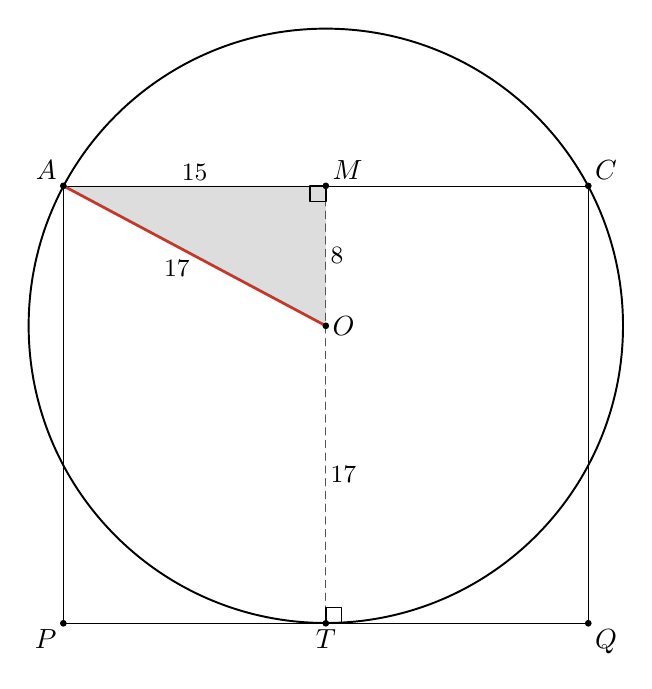
\begin{tikzpicture}
%! let R = 17
\tkzDefPoint(0.0,0.0){P} %! P = (0, 0)
\tkzDefPoint(6.6666667,0.0){Q} %! Q = (30, 0)
\tkzDefPoint(0.0,5.5555556){A} %! A = (0, 25)
\tkzDefPoint(6.6666667,5.5555556){C} %! C = (30, 25)
\tkzDefPoint(3.3333333,5.5555556){M} %! M = mid(A, C)
\tkzDefPoint(3.3333333,0.0){T} %! T = mid(P, Q)
\tkzDefPoint(3.3333333,3.7777778){O} %! O = (15, R)
%! fact on_circle(A, O, R)
%! fact on_circle(C, O, R)
%! fact tangent(O, R, P, Q)
%! fact midpoint(M, A, C)
%! fact midpoint(T, P, Q)
%! fact perp(A, C, O, M)
%! fact collinear(O, M, T)
%! fact dist(A, C) == 30
%! fact dist(A, P) == 25
%! fact dist(A, M) == 15
%! fact dist(O, M) == 8
%! fact dist(O, A) == 17
%! fact dist(O, T) == 17
\tkzFillPolygon[color=figtint](A,M,O)
\tkzDrawCircle(O,A)
\tkzDrawPolygon(A,C,Q,P)
\tkzDrawSegment[aux](M,T)
\tkzDrawSegment[key](O,A)
\tkzMarkRightAngle[size=.2,mk](A,M,O)
\tkzMarkRightAngle[size=.2,mk](Q,T,O)
\tkzDrawPoints(A,C,P,Q,M,T,O)
\tkzLabelPoint[above left,lbl](A){$A$}
\tkzLabelPoint[above right,lbl](C){$C$}
\tkzLabelPoint[below left,lbl](P){$P$}
\tkzLabelPoint[below right,lbl](Q){$Q$}
\tkzLabelPoint[above right,lbl](M){$M$}
\tkzLabelPoint[below,lbl](T){$T$}
\tkzLabelPoint[right,lbl](O){$O$}
\tkzLabelSegment[above,pos=.5,len](A,M){$15$}
\tkzLabelSegment[right,pos=.5,len](M,O){$8$}
\tkzLabelSegment[right,pos=.5,len](O,T){$17$}
\tkzLabelSegment[below left,pos=.5,len](O,A){$17$}
\end{tikzpicture}
\end{document}
